\chapter{Comparison with QUIJOTE-MFI Data}\label{ch:comparison_quijote}

In this chapter values of atmospheric brightness temperature, which have
been obtained making use of the numerical methods described in
\autoref{ch:statistical_picture} and \autoref{ch:atm_variations}, are
compared with measurements acquired by the QUIJOTE experiment.

In particular, the values of $T_\text{atm}$ that have been measured by the
\emph{Multi-Frequency Instrument} (MFI) are considered. MFI is mounted on
the QT1 telescope, which is deployed at the Observatorio del Teide. It
operates since November 2012 in four bands centered at
\SIlist{11;13;17;19}{\giga\hertz}.

\section{QUIJOTE Data and Raw Simulations}

The QUIJOTE dataset is represented in \autoref{fig:quijote_dataset}.
It includes measurements from a total of \num{444} MFI \emph{sky-dip}
observations, performed between December 2012 and February 2015.  On
average, we have one observation every \num{1.78} days. However, the time
distribution of the data is quite inhomogeneous. There are periods in which
we have one observation every sidereal day (sometimes two per day), but
there are some extended periods without observations.

\begin{figure}
        \centering
        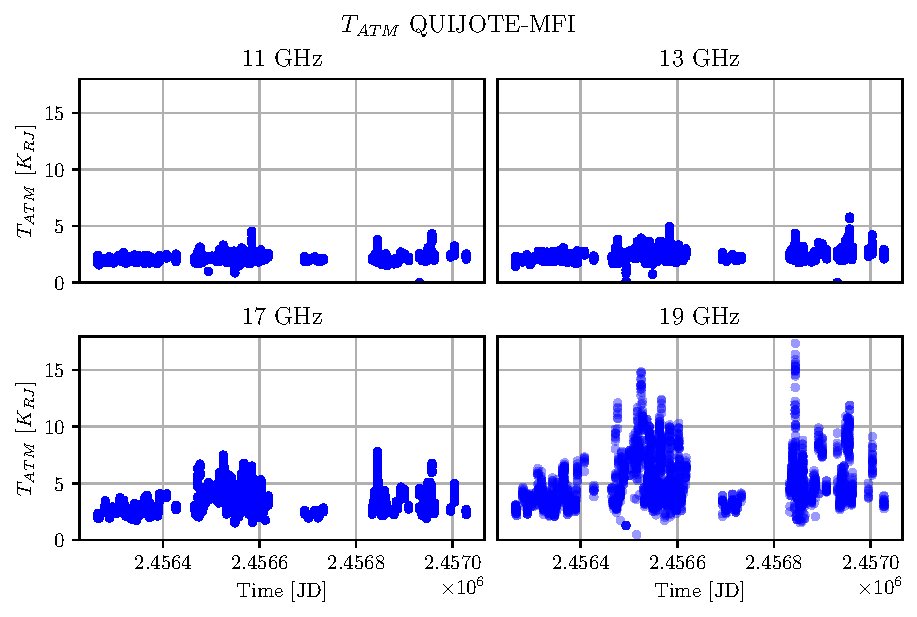
\includegraphics[width=\textwidth]{QUIJOTE_Dataset}
        \caption{QUIJOTE-MFI  $T_{atm}$ dataset.}
        \label{fig:quijote_dataset}
\end{figure}

For each point of the scatter plot showed in \autoref{fig:quijote_dataset},
we have used CAL to simulate a value of atmospheric brightness temperature
at the same frequency and at the same hour of a typical day of the
corresponding month. The comparison between simulated data and
$T_\text{atm}$ acquired by the QUIJOTE-MFI instrument is showed in
\autoref{fig:quijote_sim}.

\begin{figure}
        \centering
        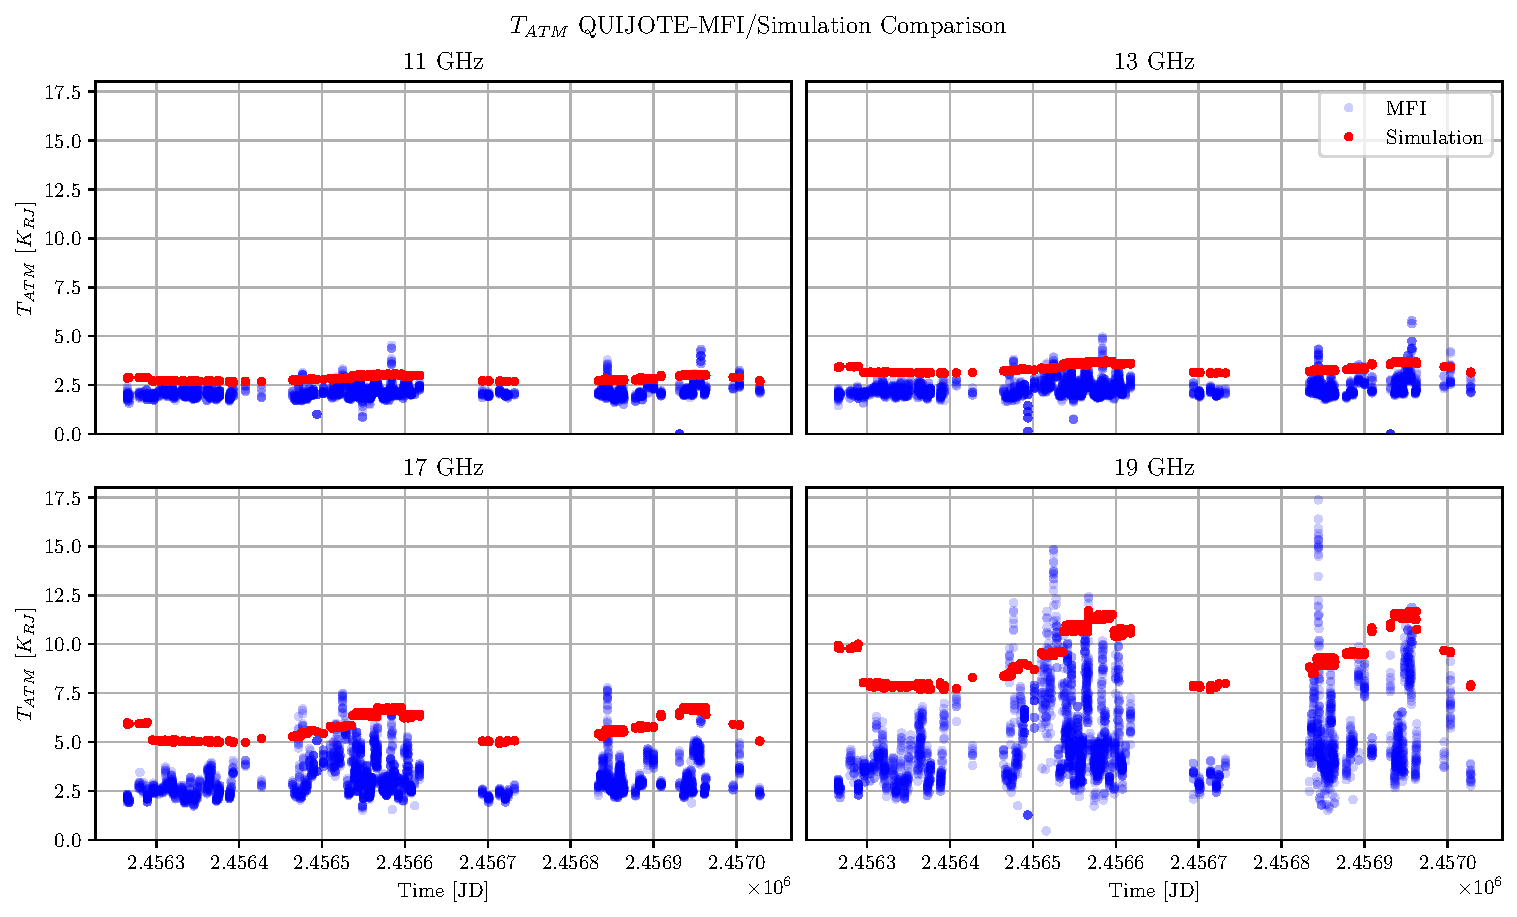
\includegraphics[width=\textwidth]{QUIJOTE-Sim}
        \caption{Comparison between QUIJOTE-MFI measurements and CAL
        simulated data.}
        \label{fig:quijote_sim}
\end{figure}

The scatter plot shows that a significant mismatch occurs. In particular
the simulations performed with CAL, making use of ERA5 dataset, yield higher
values of atmospheric brightness temperature. The mismatch becomes
especially problematic for higher frequencies, approaching the
\SI{22}{\giga\hertz} water vapour line. Moreover, QUIJOTE-MFI data
exhibit much greater fluctuations over time.

We recognise that part of the issues showed in \autoref{fig:quijote_sim}
are due to the insufficient spatial resolution of ERA5 reanalysis data.
\autoref{fig:pwv_teide_1980-01-01_12-00} shows a focus on the pixel in
which the Observatorio del Teide is located. In particular we are
interested in the area in which the Strip telescope will be deployed, which
in the figure is signaled by a red circle. The ERA5 dataset only provides a
single value per hour of the PWV for the whole pixel, which constitutes a
spatial average.  Therefore, values of PWV are biased by contributions from
coastal low lands, below \SI{2390}{\meter}, and ocean waters. In other
words, the total column water vapour values that have been taken into
account to evaluate atmospheric brightness temperatures greatly exceeds
true values for Pico del Teide.

\begin{figure}
        \centering
        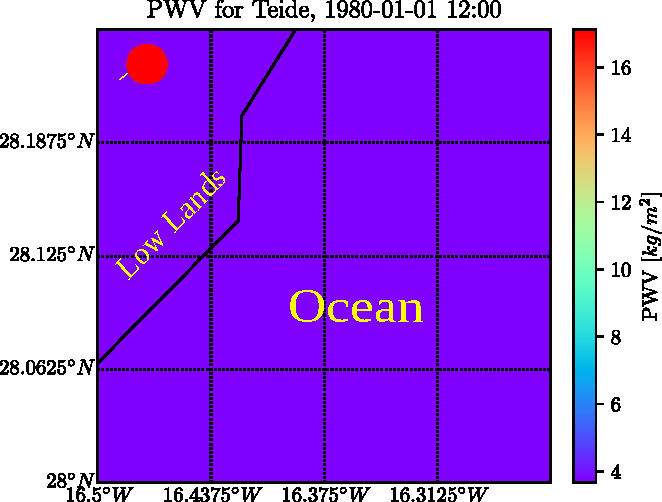
\includegraphics[width=0.80\textwidth]{PWV_Teide_1980-01-01_12-00}
        \caption{PWV for Pico del Teide.}
        \label{fig:pwv_teide_1980-01-01_12-00}
\end{figure}

\section{The Calibration Coefficient}

\begin{figure}
        \centering
        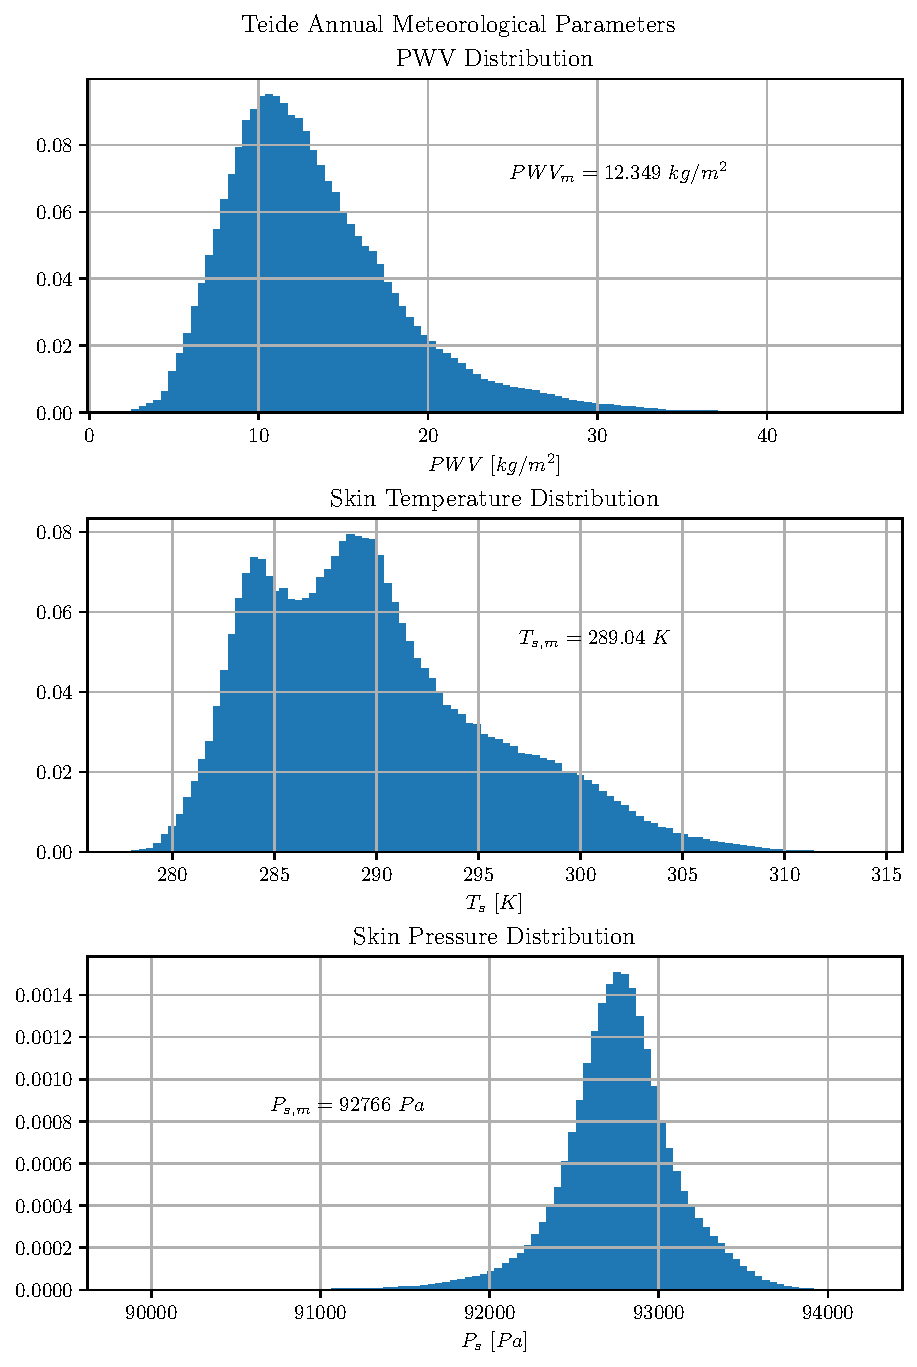
\includegraphics[width=0.93\textwidth]{Teide_Annual_Distributions}
        \caption{Annual distribution for relevant meteorological parameters
        at Pico del Teide.}
        \label{fig:teide_annual_distributions}
\end{figure}

\begin{figure}
        \centering
        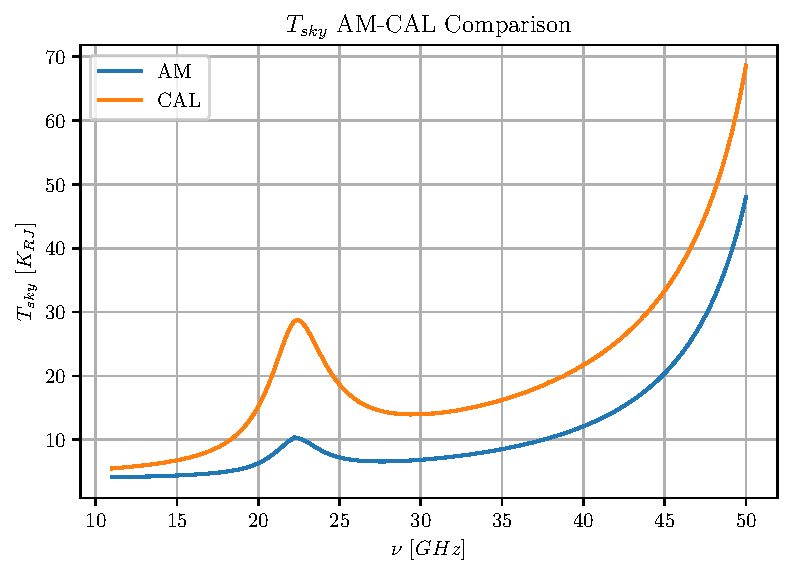
\includegraphics[width=\textwidth]{AM_CAL_Comparison}
        \caption{AM/CAL sky brightness temperatures comparison.}
        \label{fig:am_cal_comparison}
\end{figure}

\begin{figure}
        \centering
        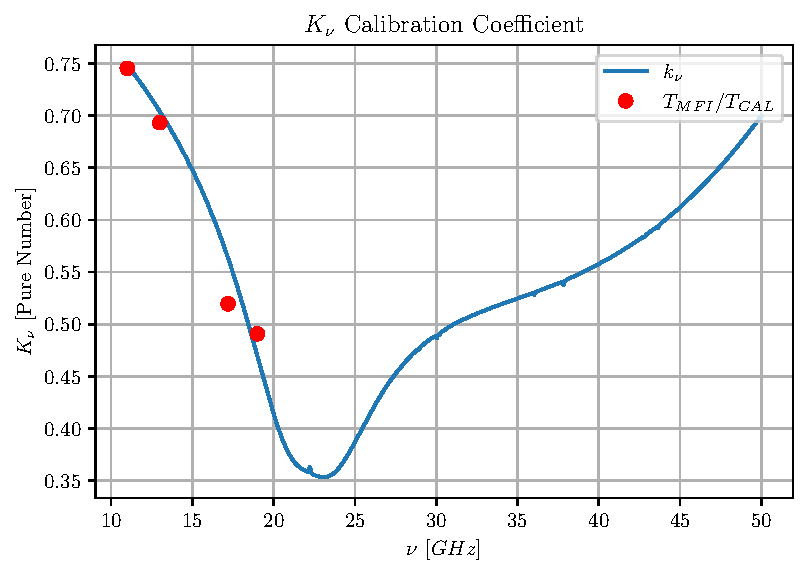
\includegraphics[width=\textwidth]{Calibration_Coefficient_QUIJOTE}
        \caption{$K_\nu$ calibration coefficient.}
        \label{fig:calibration_coefficient_quijote}
\end{figure}

\section{Comparison with Calibrated Data}

\begin{figure}
        \centering
        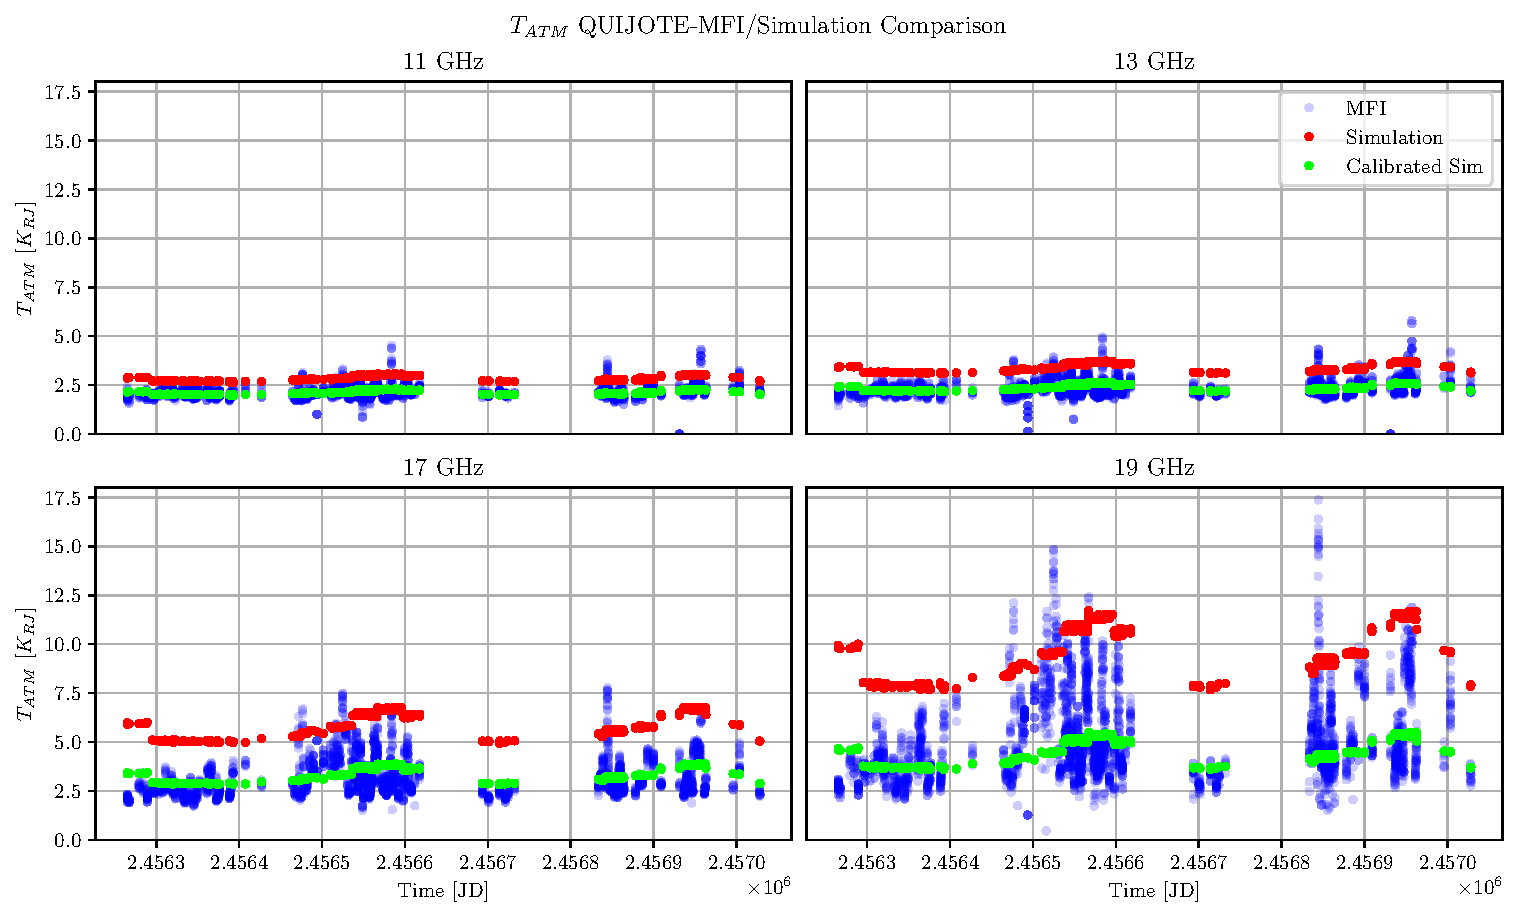
\includegraphics[width=\textwidth]{QUIJOTE-Sim_calibrated}
        \caption{Comparison between QUIJOTE-MFI measurements and
        CAL simulated data with calibration applied.}
        \label{fig:quijote_sim_calibrated}
\end{figure}

